%%%%%%%%%%%%%%%%%%%%%%%%%%%%%%%%%%%%%%%%%
% Masters/Doctoral Thesis 
% LaTeX Template
% Version 2.4 (22/11/16)
%
% This template has been downloaded from:
% http://www.LaTeXTemplates.com
%
% Version 2.x major modifications by:
% Vel (vel@latextemplates.com)
%
% This template is based on a template by:
% Steve Gunn (http://users.ecs.soton.ac.uk/srg/softwaretools/document/templates/)
% Sunil Patel (http://www.sunilpatel.co.uk/thesis-template/)
%
% Template license:
% CC BY-NC-SA 3.0 (http://creativecommons.org/licenses/by-nc-sa/3.0/)
%
%%%%%%%%%%%%%%%%%%%%%%%%%%%%%%%%%%%%%%%%%

%----------------------------------------------------------------------------------------
%	PACKAGES AND OTHER DOCUMENT CONFIGURATIONS
%----------------------------------------------------------------------------------------

\documentclass[
11pt, % The default document font size, options: 10pt, 11pt, 12pt
%oneside, % Two side (alternating margins) for binding by default, uncomment to switch to one side
english, % ngerman for German
singlespacing, % Single line spacing, alternatives: onehalfspacing or doublespacing
%draft, % Uncomment to enable draft mode (no pictures, no links, overfull hboxes indicated)
%nolistspacing, % If the document is onehalfspacing or doublespacing, uncomment this to set spacing in lists to single
%liststotoc, % Uncomment to add the list of figures/tables/etc to the table of contents
%toctotoc, % Uncomment to add the main table of contents to the table of contents
%parskip, % Uncomment to add space between paragraphs
%nohyperref, % Uncomment to not load the hyperref package
headsepline, % Uncomment to get a line under the header
%chapterinoneline, % Uncomment to place the chapter title next to the number on one line
%consistentlayout, % Uncomment to change the layout of the declaration, abstract and acknowledgements pages to match the default layout
]{MastersDoctoralThesis} % The class file specifying the document structure

\usepackage[utf8]{inputenc} % Required for inputting international characters
\usepackage[T1]{fontenc} % Output font encoding for international characters

\usepackage{palatino} % Use the Palatino font by default

\usepackage{color}
\usepackage{amssymb}
\usepackage{amsmath}

\usepackage[backend=bibtex,style=authoryear,natbib=true]{biblatex} % Use the bibtex backend with the authoryear citation style (which resembles APA)

\addbibresource{example.bib} % The filename of the bibliography

\usepackage[autostyle=true]{csquotes} % Required to generate language-dependent quotes in the bibliography

%----------------------------------------------------------------------------------------
%	MARGIN SETTINGS
%----------------------------------------------------------------------------------------

\geometry{
	paper=a4paper, % Change to letterpaper for US letter
	inner=2.5cm, % Inner margin
	outer=3.8cm, % Outer margin
	bindingoffset=.5cm, % Binding offset
	top=1.5cm, % Top margin
	bottom=1.5cm, % Bottom margin
	%showframe, % Uncomment to show how the type block is set on the page
}

%----------------------------------------------------------------------------------------
%	THESIS INFORMATION
%----------------------------------------------------------------------------------------

\thesistitle{Efficient Target Identification during Haptic Search in a Three-dimensional Environment} % Your thesis title, this is used in the title and abstract, print it elsewhere with \ttitle
\supervisor{} % Your supervisor's name, this is used in the title page, print it elsewhere with \supname
\examiner{} % Your examiner's name, this is not currently used anywhere in the template, print it elsewhere with \examname
\degree{Bachelor of Science} % Your degree name, this is used in the title page and abstract, print it elsewhere with \degreename
\author{Julian Nowainski} % Your name, this is used in the title page and abstract, print it elsewhere with \authorname
\addresses{} % Your address, this is not currently used anywhere in the template, print it elsewhere with \addressname

\subject{} % Your subject area, this is not currently used anywhere in the template, print it elsewhere with \subjectname
\keywords{} % Keywords for your thesis, this is not currently used anywhere in the template, print it elsewhere with \keywordnames
\university{\href{http://www.uni-bielefeld.de}{University of Bielefeld}} % Your university's name and URL, this is used in the title page and abstract, print it elsewhere with \univname
\department{CITEC} % Your department's name and URL, this is used in the title page and abstract, print it elsewhere with \deptname
\group{\href{https://ni.www.techfak.uni-bielefeld.de/}{Neuroinformatics Group}} % Your research group's name and URL, this is used in the title page, print it elsewhere with \groupname
\faculty{\href{http://faculty.university.com}{Faculty of Technology}} % Your faculty's name and URL, this is used in the title page and abstract, print it elsewhere with \facname

\AtBeginDocument{
\hypersetup{pdftitle=\ttitle} % Set the PDF's title to your title
\hypersetup{pdfauthor=\authorname} % Set the PDF's author to your name
\hypersetup{pdfkeywords=\keywordnames} % Set the PDF's keywords to your keywords
}

\begin{document}

\frontmatter % Use roman page numbering style (i, ii, iii, iv...) for the pre-content pages

\pagestyle{plain} % Default to the plain heading style until the thesis style is called for the body content

%----------------------------------------------------------------------------------------
%	TITLE PAGE
%----------------------------------------------------------------------------------------

\begin{titlepage}
\begin{center}

\vspace*{.06\textheight}
{\scshape\LARGE \univname\par}\vspace{1.5cm} % University name
\textsc{\Large Bachelor Thesis}\\[0.5cm] % Thesis type

\HRule \\[0.4cm] % Horizontal line
{\huge \bfseries \ttitle\par}\vspace{0.4cm} % Thesis title
\HRule \\[1.5cm] % Horizontal line
 
\begin{minipage}[t]{0.4\textwidth}
\begin{flushleft} \large
\emph{Author:}\\
\href{}{\authorname} % Author name - remove the \href bracket to remove the link
\end{flushleft}
\end{minipage}
\begin{minipage}[t]{0.4\textwidth}
\begin{flushright} \large
\emph{Supervisor:} \\
\href{}{\supname} % Supervisor name - remove the \href bracket to remove the link  
\end{flushright}
\end{minipage}\\[3cm]
 
\vfill

\large \textit{A thesis submitted in fulfillment of the requirements\\ for the degree of \degreename}\\[0.3cm] % University requirement text
\textit{in the}\\[0.4cm]
\groupname\\\deptname\\[2cm] % Research group name and department name
 
\vfill

{\large \today}\\[4cm] % Date
%\includegraphics{Logo} % University/department logo - uncomment to place it
 
\vfill
\end{center}
\end{titlepage}

%----------------------------------------------------------------------------------------
%	DECLARATION PAGE
%----------------------------------------------------------------------------------------

\begin{declaration}
\addchaptertocentry{\authorshipname} % Add the declaration to the table of contents
\noindent I, \authorname, declare that this thesis titled, \enquote{\ttitle} and the work presented in it are my own. I confirm that:

\begin{itemize} 
\item This work was done wholly or mainly while in candidature for a research degree at this University.
\item Where any part of this thesis has previously been submitted for a degree or any other qualification at this University or any other institution, this has been clearly stated.
\item Where I have consulted the published work of others, this is always clearly attributed.
\item Where I have quoted from the work of others, the source is always given. With the exception of such quotations, this thesis is entirely my own work.
\item I have acknowledged all main sources of help.
\item Where the thesis is based on work done by myself jointly with others, I have made clear exactly what was done by others and what I have contributed myself.\\
\end{itemize}
 
\noindent Signed:\\
\rule[0.5em]{25em}{0.5pt} % This prints a line for the signature
 
\noindent Date:\\
\rule[0.5em]{25em}{0.5pt} % This prints a line to write the date
\end{declaration}

\cleardoublepage

%----------------------------------------------------------------------------------------
%	QUOTATION PAGE
%----------------------------------------------------------------------------------------


%----------------------------------------------------------------------------------------
%	ABSTRACT PAGE
%----------------------------------------------------------------------------------------

\begin{abstract}
\addchaptertocentry{\abstractname} % Add the abstract to the table of contents

\end{abstract}

%----------------------------------------------------------------------------------------
%	ACKNOWLEDGEMENTS
%----------------------------------------------------------------------------------------

%----------------------------------------------------------------------------------------
%	LIST OF CONTENTS/FIGURES/TABLES PAGES
%----------------------------------------------------------------------------------------

\tableofcontents % Prints the main table of contents

%\listoffigures % Prints the list of figures

%\listoftables % Prints the list of tables

%----------------------------------------------------------------------------------------
%	ABBREVIATIONS
%----------------------------------------------------------------------------------------



%----------------------------------------------------------------------------------------
%	PHYSICAL CONSTANTS/OTHER DEFINITIONS
%----------------------------------------------------------------------------------------



%----------------------------------------------------------------------------------------
%	SYMBOLS
%----------------------------------------------------------------------------------------



%----------------------------------------------------------------------------------------
%	DEDICATION
%----------------------------------------------------------------------------------------


%----------------------------------------------------------------------------------------
%	THESIS CONTENT - CHAPTERS
%----------------------------------------------------------------------------------------

\mainmatter % Begin numeric (1,2,3...) page numbering

\pagestyle{thesis} % Return the page headers back to the "thesis" style

% Include the chapters of the thesis as separate files from the Chapters folder
% Uncomment the lines as you write the chapters

% Chapter 1

\chapter{Introduction} % Main chapter title

\label{Introduction} % For referencing the chapter elsewhere, use \ref{Chapter1} 

%----------------------------------------------------------------------------------------

% Define some commands to keep the formatting separated from the content 
\newcommand{\keyword}[1]{\textbf{#1}}
\newcommand{\tabhead}[1]{\textbf{#1}}
\newcommand{\code}[1]{\texttt{#1}}
\newcommand{\file}[1]{\texttt{\bfseries#1}}
\newcommand{\option}[1]{\texttt{\itshape#1}}

%----------------------------------------------------------------------------------------
\section{Motivation}
Humans are very skilled when it comes to the task of exploring objects based merely on the haptic feedback they get from touching them. In a setting with multiple objects, a desired object can be found quite fast among the others. Searching for some objects like keys in a bag, or a phone on a nightstand in the dark are some examples of a three-dimensional haptic search task. In such tasks, one searches for a desired object, called the target, amongst other objects that are not of interest called distractors. Often, it is a specific feature of an object that makes it stand out among others. These features can be, for an instance, material properties, size, weight or shape \cite{HapticShape}. This is called the pop-out effect where the target feature is then said to be salient with respect to the distractor properties. \\
This phenomenon has not only been aspect of research in the haptic domain, but rather had its beginning in the vision. An example was to find a red dot among green ones, which could be done effortlessly without the need for a throughout search. However, finding a line with a specific rotation in an image with multiple lines of various rotations takes some effort \cite{treisman_gormican_1988}. Furthermore Ledermann and Klatsky found in 1987 \cite{EPs}, that each search strategy consists of a set of patterns of explorations that are called exploratory procedures (EPs). This means that the efficiency of a haptic search is not only based on the salient target feature, but also on the search strategy that is used. This shows the complexity of haptic search tasks and makes it even more interesting that humans can do this with high accuracy and seemingly little effort.  \\
A lot of research was done to investigate human behavior in such tasks, but to this day it was merely investigated what the approaches are to implement such behavior in technical systems such as robots. This work wants to consider two questions with the data recorded in a haptic search experiment with a multimodal glove worn by participants: Is it possible to inspect these pop-out effects based on tactile data and pose-information as well as the question of the applicability of these data in machine learning tasks. 

\section{Goals} \label{Goals}
A first goal of this work was to provide a setting where haptic search tasks could be performed by participants and be recorded with suitable hardware. In section \ref{Haptic Search Experiment} the haptic search experiment will be proposed and discussed starting by the experimental setup, the execution, hardware and the overall setting.\\
After having recorded the data a second goal was aimed at generating a data set that was suitable for supervised learning tasks. These included postprocessing the raw data and generating labels for the individual trials. Section \ref{Data} describes the efforts that were made to reach this goal.\\
The last goal was to use the information collected with the data to perform machine learning tasks to investigate the differences between target- and distractor objects and measure the performance of the developed models. Section \ref{Evaluation} will describe the different experiments and models that were used to address the question for applicability of recorded data from haptic search experiments performed by humans.  

% Chapter 2

\chapter{Haptic Search Experiment} % Main chapter title

\label{Haptic Search Experiment} % For referencing the chapter elsewhere, use \ref{Haptic Search Experiment} 

%----------------------------------------------------------------------------------------
%In diesem Kapitel wird der Versuch, die benutzte Hardware , %und das komplette Setting von der Aufnahme beschrieben

%----------------------------------------------------------------------------------------
\section{Haptic Search Experiment}
\subsection{Experimental Setup}
The Modular Haptic Stimuli Board (MHSB) makes up the core part of the experiment. It is a setting with two wooden frames that hold stimuli objects. These objects are 3 x 3 cm big wooden blocks, which have a primitive three-dimensional shape on top of it or are just plane. The whole set consists of 360 blocks with 55 different shapes.\\
The first wooden frame can fit 25 objects and is used for learning a target object whereas the second frame has a capacity of 100 objects and is used for searching target objects. The stimuli are statically installed in the frames and not manipulable to allow a focus on just the search task itself (see Figure \ref{MHSBBOARDS}).\\
\\
For this experiment, a subset of stimuli was chosen, consisting of 5 different shapes and plane ones (see Figure \ref{Stimuli}). The target consists of one object and is placed central in the small frame with the rest of the space consisting of plane stimuli. The big frame contains the rest of this subset, where each shape exist 4 to 5 times, including the target. The objects were distributed mostly equally and kept the same rotation throughout the experiment. Only the distribution and the target were changed with each trial.\\

\begin{figure}[H]
	\centering
	\begin{minipage}{0.49\textwidth}
		\centering
		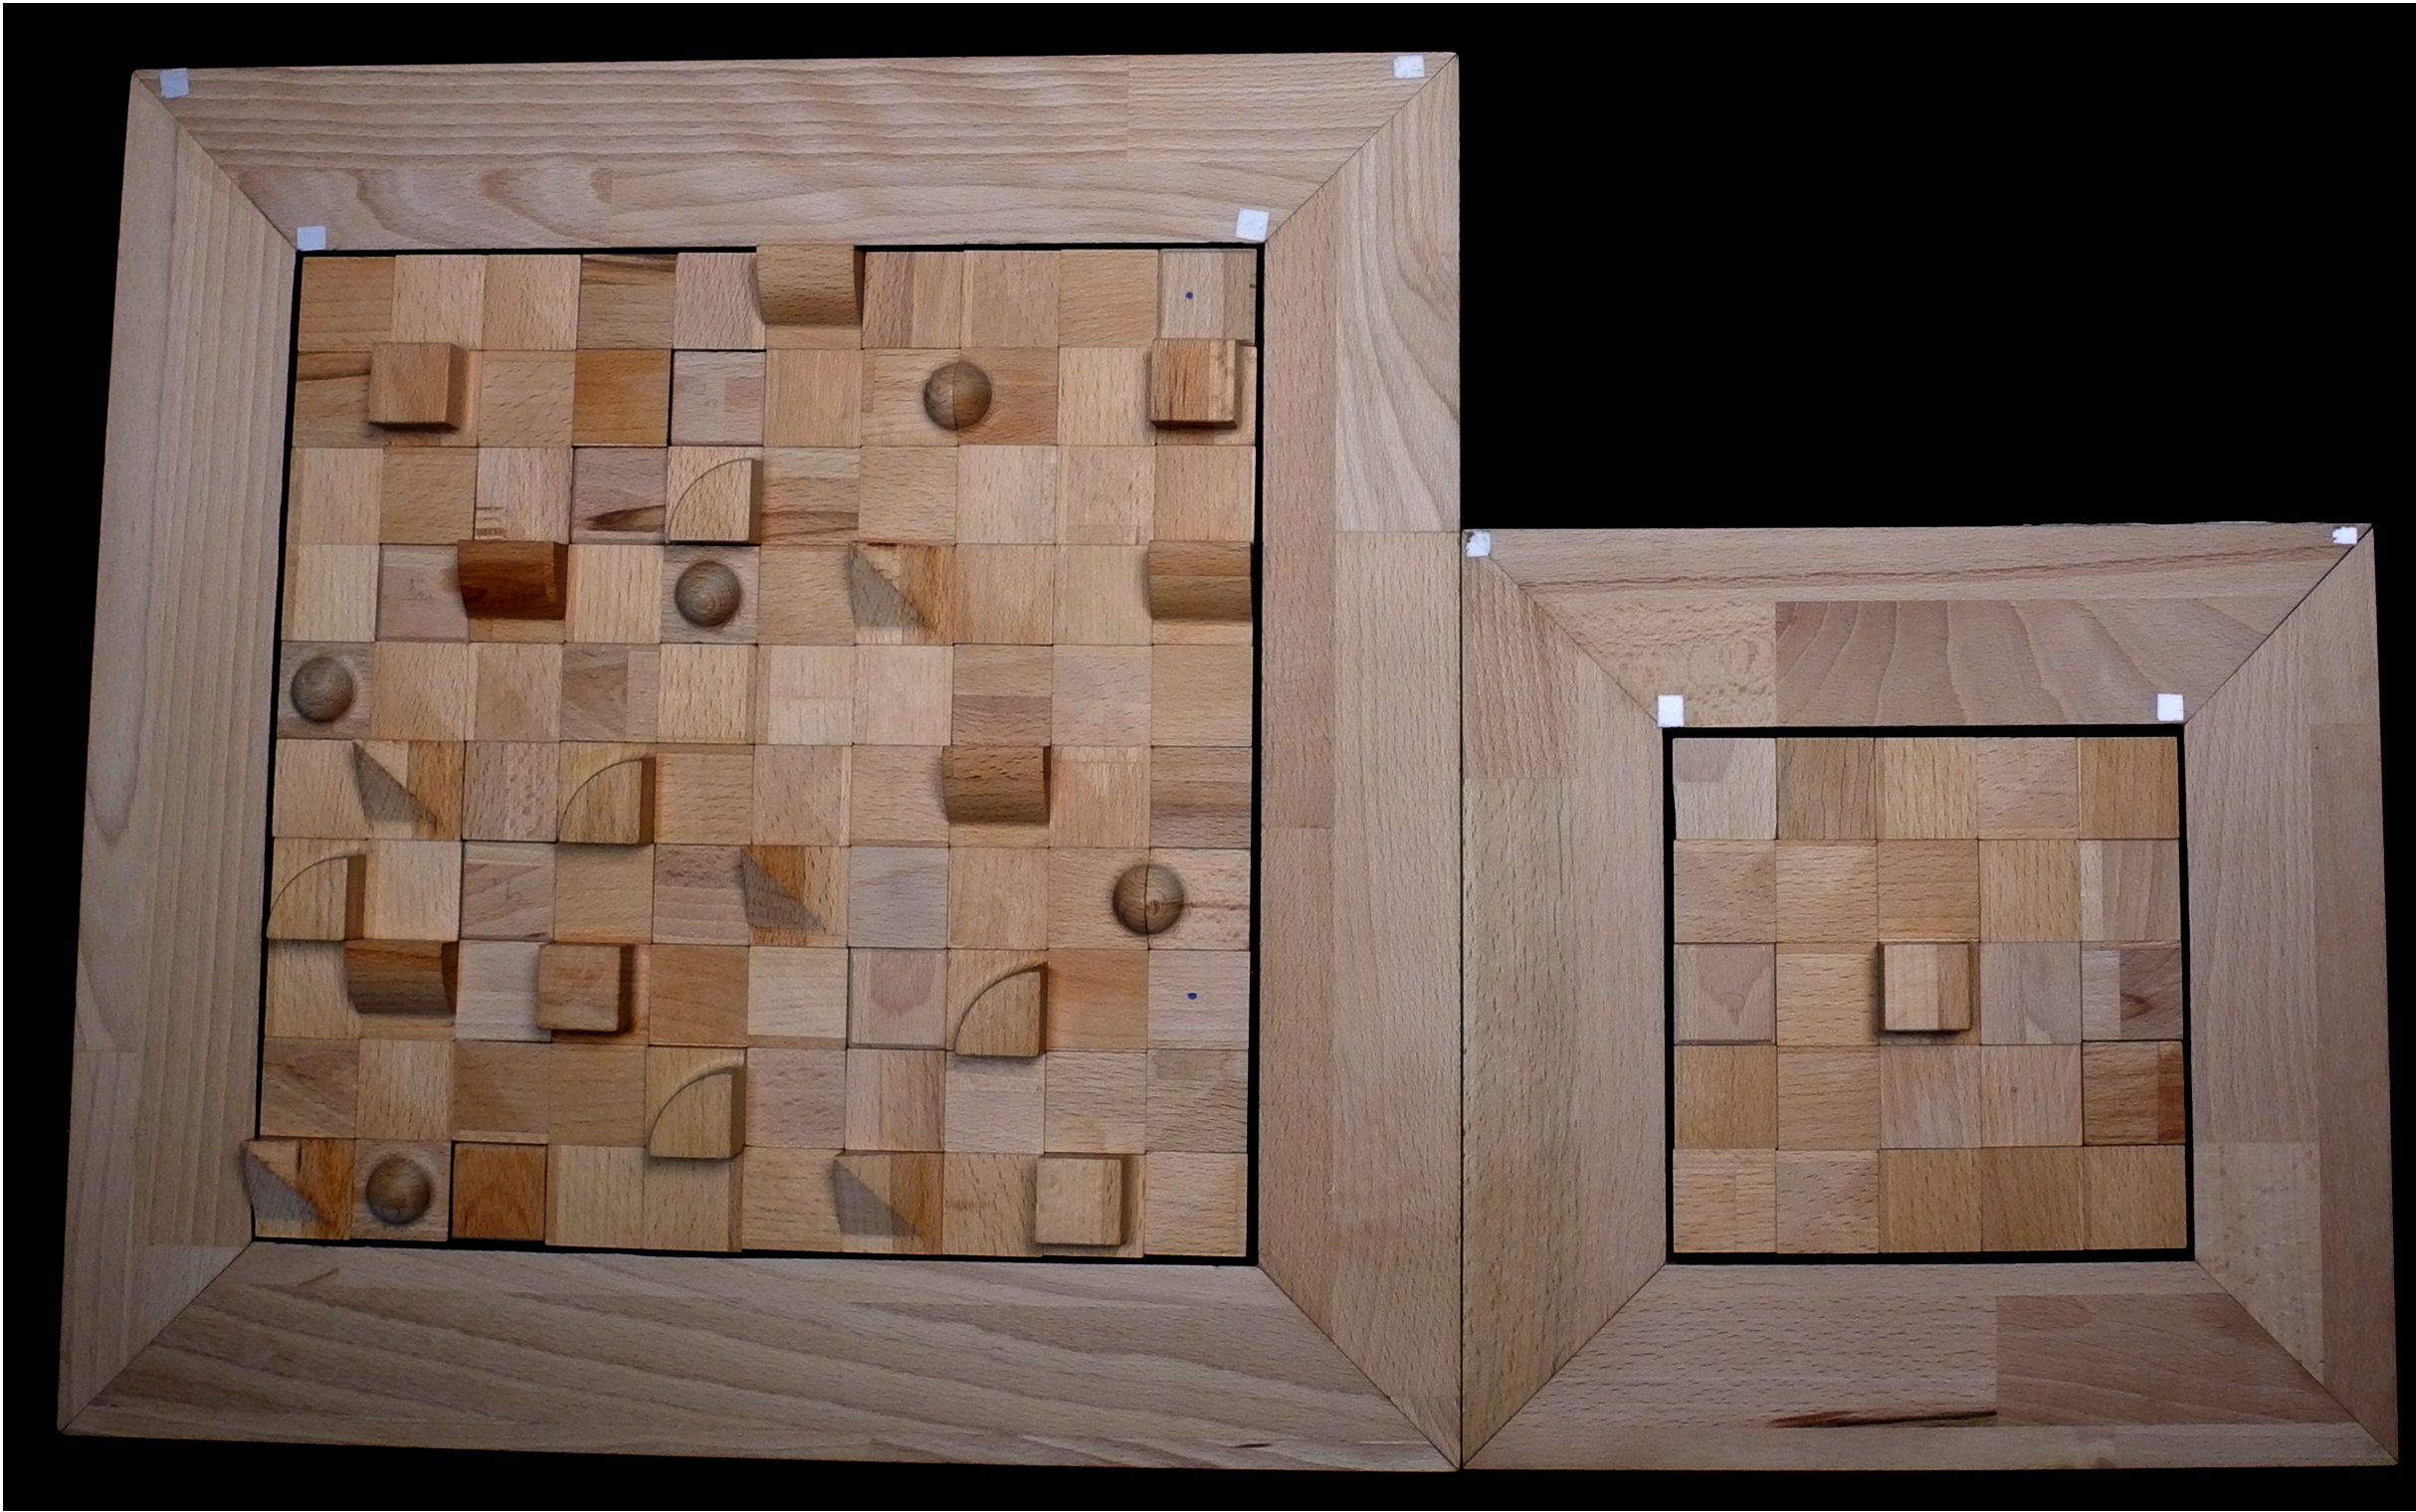
\includegraphics[width=\textwidth]{MHSB}
		\caption{MHSB: on the right side for learning, on the left for search task}
		\label{MHSBBOARDS}
	\end{minipage}
	\begin{minipage}{0.49\textwidth}
		\centering
		\includegraphics[width=0.83\textwidth]{Stimuli}
		\caption{Stimuli objects from left: Wave, Sphere, Quarter, Box, Pyramid}
		\label{Stimuli}
	\end{minipage}
\end{figure}


\subsection{Execution}  
For this experiment, 7 participants were invited and asked to solve a haptic search task while being blindfolded. The participants were 23 to 28 years old and included both genders. All participants were right-handed and have never seen the stimuli objects, so that during the task they never knew how the set of objects looked like and their perception was purely based on the haptic features.\\
Each participant performed on maximal 5 trials, where after each trial, the target was exchanged and the distribution of the stimuli on the big frame was changed. Before the beginning, there were 2 rehearsals to accustom the subjects to the setting. No participant had the same target twice or more and the task was done with just the right hand, while wearing a glove to record relevant data (See \ref{Hardware}).\\
\\
For the procedure, each participant was given a description of the task (See Appendix \ref{AppendixA}). The task consisted of two parts. \\
The first task was to explore the target object on the small frame and remembering it just by its haptic features. When collected enough information about the target stimulus, the subject should proceed to the big frame and search for the learned target. The only goal in this part was to remember the approximate position of the target and not saying that it was found or pointing at it, so the recorded data would not contain pauses or pointing postures.\\
It was not necessary to find every target shape in the big frame, just as many as one could. The time was limited to 30 seconds to guarantee that the focus lies only on the salient features. An acoustic signal by the examiner determined the start- and endpoint of the experiment.\\
The second part of the experiment was to figure out if the subjects found the target object between the non-target objects, called distractors, and how well they could remember the approximate position on the frame. Again an acoustic signal determined start and end of the trial. For the second part, the subjects had just 10 seconds left to find the targets and point on them. The short period of time was set to prevent the subjects from exploring too much of the frame and focusing only on the smallest set of haptic features that were sufficient enough to differentiate between target and distractor.\\

%----------------------------------------------------------------------------------------
\section{Hardware} \label{Hardware}
In this section the used hardware will be described as well as the overall setting that was used to record the data for the experiment.\\
There will be first a brief description of the glove that was used to capture tactile relevant and hand posture data followed by a description of the Vicon system to capture position data in a three-dimensional environment. At the end the implementation of the hardware into the experimental setting is explained.

\subsection{Glove}
A detailed explanation of the underlying technical properties and its implementation into the glove can be found in the work of Bianchi et. al. \cite{Glove}.\\
\\
To record data for this experiment, a device was needed that would be able to capture the most relevant patterns underlying a haptic search task. These so called exploratory features (EPs) describe the behavior of the hand during the exploration \cite{EPs}. Furthermore a device for recording the tactile properties was needed.\\
The multi-modal sensing glove combines both of these features. On the bottom side of the glove 64 tactile cells are mounted, covering hand palm and fingers. These fabric-based sensors record local pressures with a frequency of 150 Hz. The top side consists of 18 bending sensors, used to capture the joint angles representing the hand pose with a frequency of 50 Hz.
 
\subsection{Vicon}
For capturing the position of the hand and the MHSB, the Vicon system was used \cite{Vicon}. It records motion data with a frequency of 200 Hz, using retroreflective markers that are tracked by infrared cameras.\\
Also included is a Basler camera, generating a top-down view for the experiment.

\subsection{Setting}
To record motion data from the subjects hand, 17 reflective markers has been placed on an extra glove that the participant wears atop of the multi-modal one. The markers were placed in a position as shown in Figure \ref{Glove_markers} to guarantee a good reconstruction of the finger and hand movements.\\
The most time-consuming part was to find a setting of the Vicon cameras that would capture the reflective markers continuously, making sure to minimize the occurrence of gaps. The result is shown in Figure \ref{Setting} There were 14 Vicon cameras placed in a semicircle around the MHSB. The Basler camera was placed directly above the frames. As an addition, there were 2 cameras placed on the left and right side to record also the side-view of the experiment.\\
The glove was connected via USB and serial-port to a nearby computer. A second computer controlled the Vicon system. To simultanetly start the recording, a synchronising tool called MSS was used (See \ref{recording}).

\begin{figure}[H]
	\centering
	\begin{minipage}{0.49\textwidth}
		\centering
		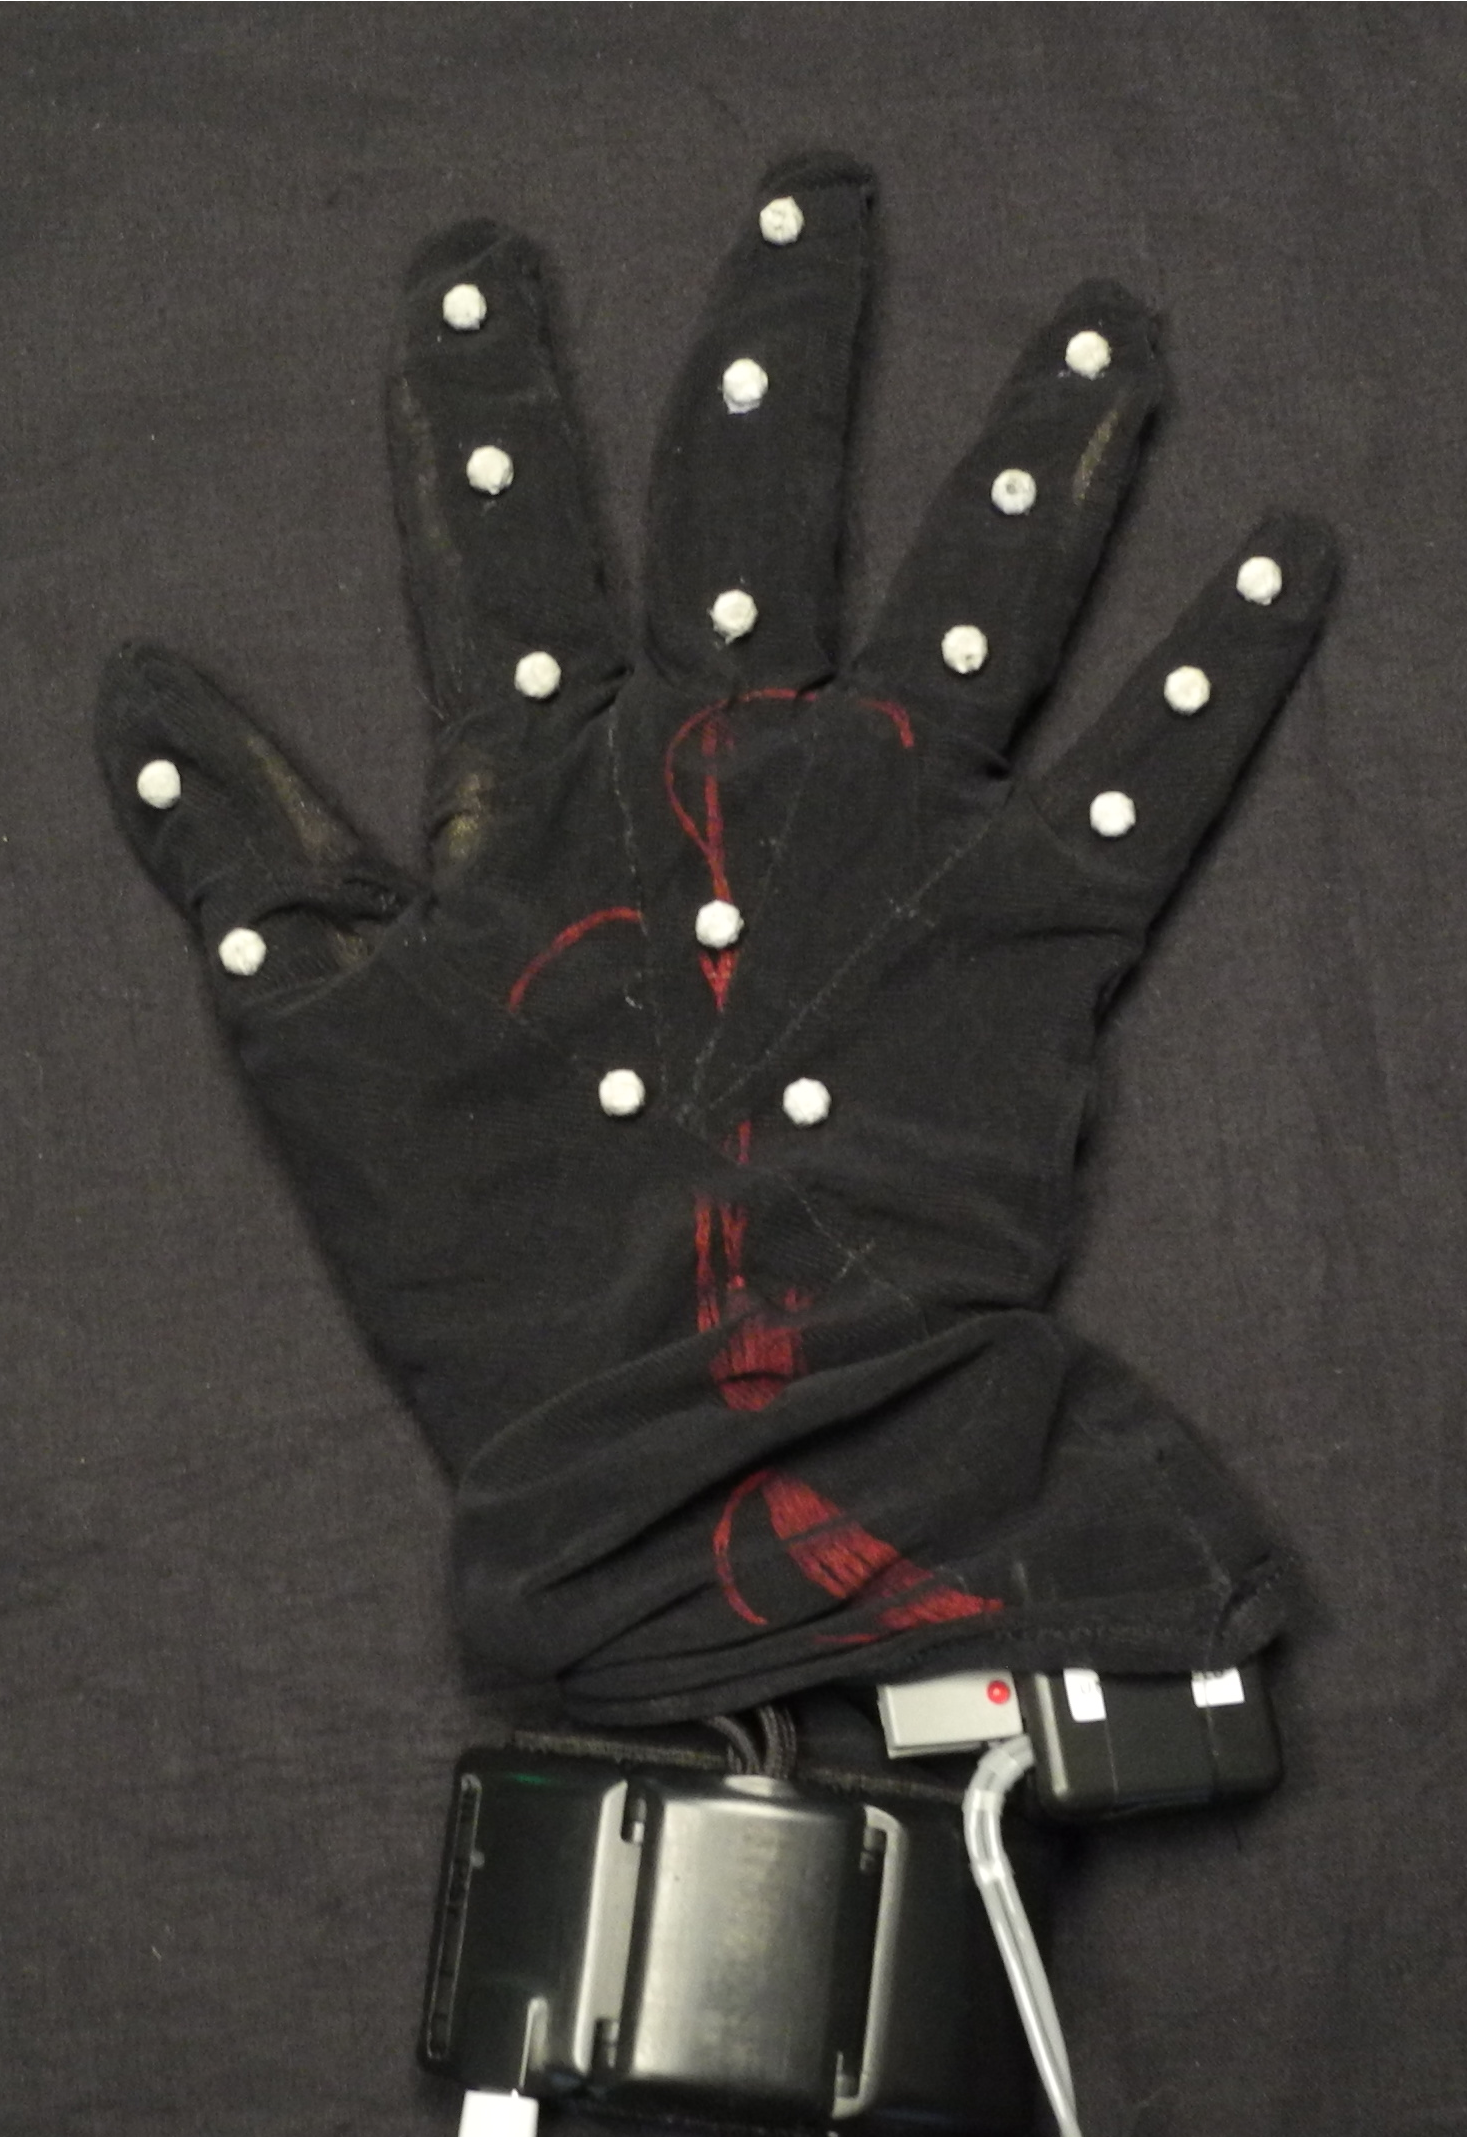
\includegraphics[width=0.55\textwidth]{glove_markers}
		\caption{Glove with 17 retroreflective markers for tracking the hand movement with Vicon}
		\label{Glove_markers}
	\end{minipage}
	\begin{minipage}{0.49\textwidth}
		\centering
		\includegraphics[width=\textwidth]{Setting}
		\caption{Experimental setting with MHSB, glove and Vicon cameras}
		\label{Setting}
	\end{minipage}
\end{figure}
  
% Chapter 3

\chapter{Data Generation and Analysis} % Main chapter title

\label{Data} % For referencing the chapter elsewhere, use \ref{Chapter1} 

%----------------------------------------------------------------------------------------
This chapter addresses the methods and efforts to tackle the task of data generation as well as labeling the huge amount of data that was recorded.\\
It was the most time-consuming part of this work, since it involved a lot of postprocessing and data cleansing work that was necessary due to the multi-modality of the recording devices and capturing data with different frequencies with various data formats which also were partly unsynchronized. Furthermore methods are explained that were used to label the generated data mostly automatically, based on position data of the hand and the MHSB, as well as a representation of the distribution of the stimuli objects on the frames.

%----------------------------------------------------------------------------------------
\section{Data Structure and Requirements}
The data in this experiment was recorded with multiple devices, including the Vicon system, the 2 parts of the glove as well as 3 cameras, generating side- and top-views. To be able to train a classifier with supervised learning, there were a number of requirements to the data:
\begin{enumerate}
\item Simultaneous data acquisition
\begin{itemize}
\item Capturing all devices at the same time will facilitate upcoming processing steps
\end{itemize}
\item Postprocessing raw data
\begin{itemize}
\item To be able to work with the data, raw data needs to be processed and all files need to be in the same format
\end{itemize}
\item Synchronizing the time-series
\begin{itemize}
\item Delays in the data acquisition and different device frequencies make this step necessary
\end{itemize}
\item Generating the labels
\begin{itemize}
\item For supervised learning, the whole dataset needs to be labeled
\end{itemize}
\end{enumerate}
%----------------------------------------------------------------------------------------
\section{Recording}
To record the data of all devices preferably at the same time and with giving just one start signal, a tool called Multiple Start Synchronizer (MSS) was used. MSS sends a trigger signal to all registered devices which makes them start and stop capturing data.\\
The Vicon and Basler camera data were captured directly within the Vicon Nexus program. For the glove, data was recorded as rosbag consisting of two topics for each part of the glove. Side-view camera images were captured directly as image files.\\
\\
Despite using MSS, there were still delays among the different devices that had to be synchronized separately. 
%----------------------------------------------------------------------------------------
\section{Postprocessing Vicon Data}
The first step in the pipeline was to postprocess the Vicon data. In this procedure, a three-dimensional hand model with marker positions was fitted to an image of the subjects hand, \textcolor{red}{see figure xyz(fitting and reconstruct)}. This model was then used to reconstruct the hand movement during the experiment to approximate marker positions that occurred during gaps in the recording when no camera captured a marker \textcolor{red}{see right side of figure xyz}.\\
\\
The resulting file contains a time-series of the x-,y- and z-position of each marker. Furthermore a file with the joint-angles was generated.
%----------------------------------------------------------------------------------------
\section{Generating Labels}
This section will describe the methodology that was used to generate labels for the recorded data. The challenge was to write a program, that will do most of the work automatically and handle the huge amount of data generated by this experiment.\\
With 7 subjects participating in up to 5 trials each, and a time series containing between 5000 and 7000 data points for each trial, a manual labeling of the data would be too time-consuming. Also having to cope with unsynchronized data due to delays between the modalities would make this task hard to tackle without proper preprocessing. The solution was a program that used the trajectories of the Vicon data to extract objects that were explored during the search experiment and to label them appropriately. The exact procedure is described in the subsections below. It can be summarized to three mandatory steps:
\begin{enumerate}
	\item Synchronizing data from Vicon and glove to allocate positions to tactile data
	\item Building a representation of the experimental setting to recreate it in sense of the hand trajectories and object distribution
	\item Generating labels by replaying these trajectories and constructing a vector containing the explored objects at each timestep
\end{enumerate}

\subsection{Synchronizing Glove and Vicon Data}
A problem that occurred during the acquisition was the delay between starting the Vicon system and the glove recording. Although sending a trigger signal to both systems at the same time, the glove started capturing data approximately 3 to 5 seconds later. Additionally the beginning of the Vicon data had to be cut by 100 to 1000 frames for postprocessing reasons. Fitting the three-dimensional model was only successful if the markers of the first frames had a nearly perfect plane position. As a consequence, an offset had to be defined pointing to the beginning of the Vicon time series because the data only contains a timestamp describing the beginning of the recording. On the other hand the recorded rosbags from the glove came with a timestamp for each sample.\\
Since the frequency of the tactile glove with 150 Hz is lower than the frequency of Vicon with 200 Hz, the trajectory data should be reduced to the length of the tactile glove.\\
\\
Consider we have two time series $V = \{v_{t} \mid t\in T_{V}\}$ and $G = \{g_{t} \mid t\in T_{G}\}$ describing the set for the Vicon data and glove data. The set of timestamps $T_{G}$ was given for the tactile data and consisting of unix time values. For $T_{V}$ the timestamps had to be calculated for each sample from the initial timestamp, the offset and the frequency. \\
To synchronize, a new time series $V' \subset V$ was defined with \begin{center}
$V' = \{v_{t} \mid \forall g_{t_{g}} \in G \exists v_{t_{v}} \in V : t_{v} \geq t_{g} \wedge t_{v} < t_{g+1}, t_{v} \in T_{V}, t_{g} \in T_{G} \}$
\end{center}
This new time series has now equal length to $G$ and each time value from $V'$ matches exactly one time value from the time series $G$.
\subsection{Representing Glove and Objects}
The core idea behind this program was to use the hands trajectories and approximated object positions to detect which object was covered by the hand during which time. Having the trajectory data given, the only thing that had to be done manually was the object distribution. For this, a representation of the board was generated in form of a matrix $B \in \mathbb{R}^{10 \times 10}$ for each trial. In this representation, $b_{11} \in \Omega=\{0,..,5\}$ would be the top left object and from there rows and columns were generated accordingly where $\Omega$ is the set of labels. To decrease the number of false-positives, only explored objects were considered in this representation.(\textcolor{red}{see fig. with rep next to picture of MHSB})\\
The next level was to represent this information in a coordinate system by generating polygons for each object in $ B $ to embody the MHSB. Since only the top corners of the boards were assembled with markers, the positions for respective corners of the polygons had to be calculated based on this. First for each object $ b_{ij} \in B $ a polygon $ P_{ij} = \begin{pmatrix}a & b \\ c & d\end{pmatrix} $ was created where each element describes the x- and y-position of a corner. In the second step, this polygon was represented as its center position $ z = \begin{pmatrix}
z_{x} \\ z_{y}
\end{pmatrix}$. The result is a matrix $B' = \begin{pmatrix}
z_{11} & \hdots & z_{1n} \\
\vdots & \ddots & \vdots \\
z_{n1} & \hdots & z_{nn}
\end{pmatrix}$
that represents every object in $ B $ through a position.\\
\\
The remaining problem was that we used the top left position of the bigger frame as a base to build our polygons using a step size corresponding to the edge length of the stimuli. As a result, the represented board was placed parallel to the x- and y-axis into the coordinate system. Because this did not match the real setting, the matrix $ B' $ had to be rotated. For this the actual angle $ \alpha $ between the vector $\vec{t} = \mu_{tr} - \mu_{tl}$, where $\mu_{tl}$ is the mean position of the top left corner and $\mu_{tr}$ the mean position of the top right corner,  and the x-axis had to be calculated to build a rotation matrix $ R_{\alpha} $. The angle $\alpha$ describes the angle with whom we need to rotate the representation so that the orientation of $ B' $ matches the one in the real setting. The final matrix for the stimuli representation is $ B''  = \begin{pmatrix}
 R_{\alpha}z_{11} & \hdots &  R_{\alpha}z_{1n} \\
\vdots & \ddots & \vdots \\
 R_{\alpha}z_{n1} & \hdots &  R_{\alpha}z_{nn}
\end{pmatrix}$.\\
\\
\\
With $ B'' $ a matrix was now given that could be used for assigning objects, or in this case their labels, to hand positions. But in order to do this, a representation for the hand had to be thought of. For now, the hand consisted of 17 trajectories $ t_{i} $, one for each marker $ i $. \\
A first approach was to use a convex hull $ H_{c} $ of the hand as seen in figure \textcolor{red}{(figure with shapes representing hand)} and check for each time step in $ V' $ if $ H_{c} $ contained points $ p \in B'' $. This idea was discarded quickly because the seize of the convex hull was to large, resulting in multiple possible objects $ p $ for each time step. Furthermore it was computationally costly since for every step the whole matrix $ B'' $ had to be checked for contained points. This led to an extension of $ B'' $ to save its elements in a k-d-tree.\\
The second approach simplified the representation by only using finger markers. Instead of the convex hull for the whole hand, the trajectories $ t_{i} $ were averaged for each finger, resulting in only 5 positions and a representation $ H'_{c} $. Also there were no checks for points $ p \in B'' $ that were contained in the convex hull anymore, but rather finding the point $ p_{i} $ with minimum distance to the center of $ H'_{c} $. These distances could be looked up now efficiently in the k-d-tree and there were no multiple possible objects for each time step but only one. This approach improved the performance greatly so that only a few points were still labeled falsely due to the size of $ H'_{c} $.\\
The last approach was fine tuned by simplifying even more. Now only three fingers were used, the index-, middle- and ring finger. Observations showed, that the little finger wasn't used often during exploration. Moreover the thumb played a redundant role, since it never touched a stimuli alone but instead together with index-, or middle finger to apply pressure. Removing the trajectories from these fingers resulted in a pyramid-like polygon that was precise enough to exclude false labels almost completely.       
 
  

\subsection{Finding Labels}
%----------------------------------------------------------------------------------------
\section{Analyzing the Data}
% Chapter 4

\chapter{Evaluation} % Main chapter title

\label{Evaluation} % For referencing the chapter elsewhere, use \ref{Chapter1} 
%----------------------------------------------------------------------------------------
\begin{text}
Hier muss ich mir noch Gedanken über das Model machen, auch was das Preprocessing angeht. In diesem Kapitel wird wahrscheinlich noch einiges umgebaut
\end{text}
\section{Model}

\section{Preprocessing}

\section{Training} 
% Chapter 5

\chapter{Evaluation} % Main chapter title

\label{Evaluation} % For referencing the chapter elsewhere, use \ref{Chapter1} 
%----------------------------------------------------------------------------------------
This chapter will present the evaluation and results of the goals that were set in \ref{Goals}.\\
At first, approaches will be explained to evaluate the goals and related work will be presented. After this, the methods are proposed containing the preprocessing steps and the selection of the training and validation sets with respect to the different approaches. In the last step, results are presented and discussed.


%----------------------------------------------------------------------------------------
\section{Approaches} \label{approaches}
In this work there were three approaches to analyze the influence of object roles in the haptic search experiment. For all of them supervised machine learning was used resulting in three different classification problems: \\
\begin{enumerate}
	\item \textbf{Classifying data into object categories:} a model was build to classify the five stimuli used in the experiment. At first the model was trained only on the data of objects when they were targets, and second on the data when they were distractors. The performance was measured and compared. The goal was to see if the data would be separable at all and to find a fitting model for it.
	
	\item \textbf{Classifying a single object as either target or distractor:} based on the previous problem, same model was trained separately for each object to classify its data into a target role or a distractor role. 
	
	\item \textbf{Classifying whole data into roles:} in this problem, the model was trained on all data to classify targets and distractors in general. The goal was to see if regardless of the object, data can be separated into target or distractor class.       
\end{enumerate}

Combining the results of all these problems, an answer to the question whether humans explore same objects differently in a haptic search task depending on what the target is should be given. Furthermore an approach to explain the human efficiency could be made by the results. Instead of classifying all explored objects, they distinguish just between two classes, the target object they searched for and a distractor.      
%----------------------------------------------------------------------------------------
\section{Related Work}
This work combines both, object categorization based on their various characteristics and haptic search. Researchers have dealt with the specific task of object classification in previous studies. Since material and functional properties could not be captured because the stimuli used were static and not deformable objects, previous work on shape based classification is perhaps the most related work to the proposed approaches.\\
Schneider et. al. \cite{Schneider} use touch sensors in a manipulation robots fingertips to gain low-resolution intensity images from multiple grasping interactions. They apply a bag-of-words approach and clustering techniques to categorize objects based on haptic feedback. Navarro et. al. presents an approach for haptic recognition and evaluation on multi-fingered robot hands based on extracting key features of tactile and kinesthetic data using clustering \cite{Navarro}. Faldella et. al \cite{Faldella} describes an approach to robotic haptic recognition using an unsupervised Kohonen self-organizing feature map for performing a match-to-sample classification of three-dimensional objects. Pezzementi et. al.views tactile sensor data as images and applies PCA techniques to identify principal components of identified features and clusters them as well as build per-class histograms as class characteristics \cite{Pezzementi}. Gorges et. al. \cite{Gorges} additionally includes passive joints in the tactile sensor system which could help to acquire more information for shape reconstructionn. They use Self-Organizing Maps for identifying haptic key features and a Bayes Classificator for classifying objects. Bhattacharjee et. al. \cite{Bhattacharjee} demonstrate a tactile sensor array covering a robot's forearm to generate haptic time series data during manipulation tasks. They use the processed and dimensionality reduced data to generate feature vectors and classify them with a k-nearest neighbor algorithm for object recognition.
\\\\
Although it is not dealt with categorization of explicit shape features in the previously defined classification problems, the tactile data acquisition, preprocessing and feature extracting used in these works could also be applied for these approaches. Especially parts of the data sampling and preprocessing pipeline from Bhattacharjee et. al. \cite{Bhattacharjee} was found to be well applicable on the data recorded for this work.

%----------------------------------------------------------------------------------------
\section{Methods}
In this section the pipeline is presented that was used for the classification problems of the evaluation. At first the preprocessing steps will be explained that will turn the raw data into feature vectors that can be used for training. Figure \ref{pipeline} depicts the complete experimental protocol. In the second part it will be described how the data sets for training and validation were generated.

\subsection{Notation}
A number of notations will be used in this work to describe the data sets that were used in the different evaluations. \\
Let $ \Omega := \{(x_{i},y_{i})\}_{i=1,...,N} $ be the data set of one trial where $ N $ is the number of samples in the time series of this trial and the tuple $ (x_{i},y_{i}) $ denotes the feature vector with the corresponding label at time $ i $. Since every trial had one target object that the participant had to search for while the rest of the objects were distractors, we can decompose the data set in $ \Omega = \Omega_{T} \cup \Omega_{D} $. Here $ \Omega_{T} $ refers to these $ (x,y) $ where $ y=t $ is label of the target object $ t \in \{1,...,5\} $ . On the other hand $ \Omega_{D} $ contains only the labels of distractor objects $ y \in \{1,...,5\}\setminus t $. A complete set $ \Omega_{A} = \Omega_{1} \cup \hdots \cup \Omega_{M} $ describes the set containing all $ M $ trials of participant $ A $.

\subsection{Preprocessing and Feature Extraction}
%\textcolor{red}{Following text has to be adapted to the new notation!}
%Tactile data was recorded from the glove with a frequency of 150Hz and joint angles at 50Hz. The classification problems were evaluated on both only the tactile data and the merged set with tactile data and joint angles. Therefore a preparation step was to sample the tactile data down to 50Hz with assigning every time value of the joint data series the corresponding tactile data vector. This will result in two time series $ T_{i} = \{x_{t} \mid t \in \{0,..,n\}\} $ and $ M_{i} = \{x_{t} \mid t \in \{0,..,m\}\} $, where $ i \in \{1,..,5\}$ describes the trial for object class $i$ and $ T,M $ refers to tactile only data or the merged set with joint angles. Each value represents a vector $x \in \mathbb{R}^{64}$ for tactile data or $ x \in \mathbb{R}^{64+18} $ for the joined set. Every component in the vector corresponds to a sensor of the 64 tactile cells or the 18 bending sensors.\\
The first step in the pipeline was to apply a z-transformation for each sensor separately with $ x_{j}' = \frac{x_{j}-\bar{x}_{j}}{\sigma_{j}} $, where $ x_{j} $ denotes the j-th component of all samples in the time series vector and $ \bar{x}_{j},\sigma_{j} $ are the mean and standard deviation. Standardizing the data to zero mean and unit variance was necessary since the different tactile cells and bending sensors all have various ranges based on the participants hand, search strategy and some noise which would significantly influence distance based classifiers.\\
Afterwards a time window was chosen to sample data from the time series at consistent intervals to reduce the amount of redundant data. The time series were recorded with 150Hz and 50Hz, resulting in very close or even similar neighboring data points. With the time window data points were picked that had a predefined time distance to the previously collected sample. In this work, a sampling rate of 10Hz proved itself reliable.\\
The next step was to extract only relevant samples dependent on the classification problem. Since one time series represents the data of a whole trial, just these data points had to be extracted that belong to specific objects, namely the ones to investigate. This had to be done individually for every approach. Only the data points that included no information at all, e.g. when the hand was in the air or outside of the MHSB, were discarded for all approaches. \\
In the last step, the extracted data was concatenated and a low dimensional representation of the data was computed using a feature extraction method. To find an optimal representation, multiple methods were applied in the first experiment and the one resulting in best performance of the model was chosen. These methods were principal component analysis (PCA) and autoencoder (AE) as well as handcrafted features like only finger sensors, the sum of the sensors on each finger and the maximum value of the sensors for each finger.

\begin{figure}[h]
	%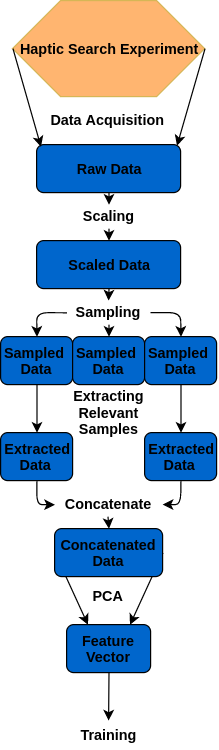
\includegraphics[scale]{Pipeline2}
	\makebox[\textwidth][c]{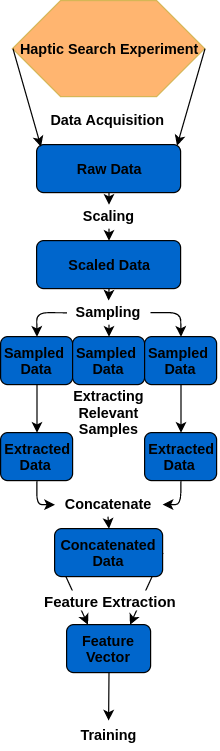
\includegraphics[scale=0.53]{Pipeline2_}}
	\caption{Schematic representation of the complete pipeline}
	\label{pipeline}
\end{figure}

\subsection{Training and Validation Methods}
%To train the feature vector for the classification problems listed in \ref{approaches}, four models were applied on the first task to measure the overall performance for object recognition and to find optimal parameters. It was trained on a k-nearest neighbor model (kNN), a multilayer perceptron (MLP), a support vector machine (SVM) and a random forest classifier. After choosing the winner model, the more specific problems were tackled with it. The results, hyperparameter and model selection is discussed in \ref{results}.\\
For training of the feature vectors and the different extraction methods, a multilayer perceptron (MLP) was applied on the data sets for the classification problems. The first experiment should serve as a baseline to see how well the data can be separated and which feature extraction would prove itself suitable. The MLP consisted of two hidden layers, was using an rectified unit activation function and the lbfgs method as an solver for weight optimization which comes from the family of quasi-Newton methods.\\
\\
A problem that occurred when recording a trial in a single run was that the whole exploration was saved in a sole data frame. This is why the extraction step in the pipeline was necessary to generate data sets suited for the classification experiment. Training was done for each participant separately and scores were averaged since high variances yielded bad results on data sets covering all participants. For the different approaches the following data was extracted to build a training and validation set:

\begin{enumerate}
	\item \textbf{Classifying data into object categories:} In fact this experiment included two sets of data. The first one was $ \Omega_{T} = \Omega_{T_{1}} \cup \hdots \cup \Omega_{T_{N}}$ which was only the data of target objects of all $ N $ trials of a participant and respectively $ \Omega_{D} = \Omega_{D_{1}} \cup \hdots \cup \Omega_{D_{N}}$. The model was trained on $ \Omega_{T} $ and $ \Omega_{D} $ independently resulting in two five-class classification problem. Comparing the performance of these sets on the models should show some insight in the information these data carries.
	%The first one was based on the data of only the target objects that had to be searched for in every trial. The second one was the inverse version where only distractor objects were extracted for each trial. Both sets included data and labels of every object in this experiment, the only difference is the role they had in the scenarios.  
	
	\item \textbf{Classifying a single object as either target or distractor:} Here a model $ M_{i} $ was trained on a set $\Omega_{i} = \Omega_{T_{i}} \cup \Omega'_{D_{j_{1}}} \cup \hdots \cup \Omega'_{D_{j_{N-1}}} $ where $ i $ describes one trial, $ \Omega_{T_{i}} $ the target data of this trial and the $ \Omega'_{D_{j_{n}}} $ describes a special case of the distractor data. Here the data for the same object that was target in trial $ i $ was extracted, but out of all other $ N-1 $ trials $ j_{n} \neq i $. Hence $ \Omega_{i} $ contains just data of one object but in the role as target and distractor. $ M_{i} $ was trained for all $i = 1,...,N $ trials and averaged to see how well the role of one object can be classified.
 	%Here the data sets were generated for every object per participant. For each stimuli and person a set was created that includes data of the object as target and as distractor. The data was labeled 1 for targets and 0 for distractor data. With the trained model it should be investigated if it is possible to distinguish the roles for same objects.   
	
	\item \textbf{Classifying whole data into roles:} For this experiment multiple sets were created and evaluated separately. The goal was to see if the roles an object can have in a haptic search could be identified from the data. First a model was trained on data $ \Omega = \Omega_{T} \cup \Omega_{D} $ where $ \Omega_{T} $ was label as 1 for all target objects and $ \Omega_{D} $ as 0 for all distractor objects combining all trials. \\
	To gain further insight into the separability of the roles, more cases were considered where the model was trained on only on target or distractor object and tested on a set with another unseen target or distractor object to test the generalization capabilities for separating roles.   
	%For this experiment a set was created containing all data points for each person. Data that representing target objects was labeled as 1 and for data representing distractors as 0. This is an extension of the previous approach, but this time it should be investigated if there are any features that make a general classification of roles independently of specific objects possible.    
\end{enumerate}  

Having generated training sets for the experiments, what was left over were suitable validation sets to test the models for generalization on unseen data. Due to the complex procedure of generating the training sets through cutting the time series for relevant objects and concatenating them back over multiple trials, some problems appeared when it came to splitting the sets for validation purpose.\\ Sampling random data points for the test set yielded almost no errors in the evaluation. Since this seemed unrealistic it was found that this was not a good way to generalize on unseen data points because even after using a time window for sampling the unprocessed data, neighboring samples were still close to each other. Also they came from exploring the same object, so this data was basically not really unseen.\\
Another approach was to use cross-validation to make sure that blocks of data that was unseen were held out for validation. However, since the data was concatenated over multiple trials this led to unseen blocks that contained whole trials which resulted in high error rates. \\
The solution was to zip the data for all trials as shown in Figure \ref{zip}. Splitting the sets of each trials into equally sized blocks and concatenating the sets blockwise resulted in an arrangement on which cross-validation could be applied. When dividing this set again into blocks and leaving one out, as it is done by cross-validation, each block would contain data from each trial. With this procedure the generalization could be tested. Splitting the trials in blocks of five and using a five-fold cross-validation on the resulting set was most suitable for the data in this work.

\begin{figure}[h]
	\makebox[\textwidth][c]{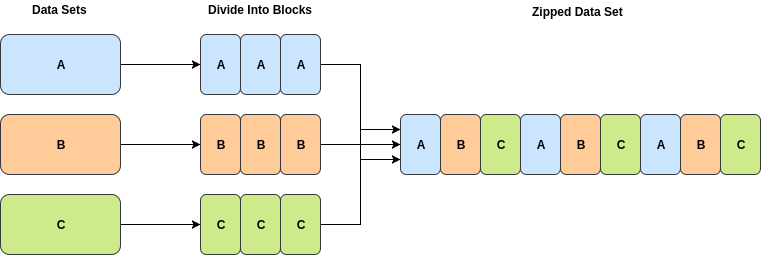
\includegraphics[scale=0.53]{Zip}}
	\caption{Schematic explanation of the zipping procedure to generate train and validation sets}
	\label{zip}
\end{figure}

\begin{table}[H]
\centering
\begin{tabular}{|c|c|}
\hline
Method & Specification \\
\hline\hline
PCA & 20 principal components \\
Autoencoder & 2 encoding layers (1 hidden), 20 features, Optimization=Adadelta, Loss=MSE\\
Finger Values & Only finger sensors used (41 features) \\
Sum Of Fingers & Sum of sensors for each finger (5 features) \\
Max Of Fingers & Max value for each finger (5 features) \\
\hline
\end{tabular}
\caption{Specifications for the used feature extraction methods}
\label{FE}
\end{table} 

\begin{table}[H]
	\centering
	\begin{tabular}{|c||c|c|c|c|c|}
		\hline
		 & Box & Sphere & Pyramid & Quarter & Wave \\
		\hline\hline
		Box & 72 (101) & 23 (7) & 6 (9) & 21 (13) & 21 (17) \\
		Sphere & 15 (9)& 70 (84) & 25 (13) & 19 (10) & 6 (5)\\
		Pyramid & 15 (7)& 15  (12)& 26 (65)& 5 (11)& 7 (8)\\
		Quarter & 37 (15)& 39 (16)& 15 (17)& 98 (183)& 6 (8)\\
		Wave & 27 (16)& 42 (15)& 0 (12)& 10 (9)& 55 (91)\\
		\hline
	\end{tabular}
	\caption{Confusion matrix for the target data set and in brackets for the distractor data set}
	\label{Confusion}
\end{table} 
%----------------------------------------------------------------------------------------
\section{Results and Discussion} \label{results}
\subsection{Classifying Data into Object Categories}\label{e2}
For this experiment the MLP was first trained and evaluated on target data and then on the set containing distractor data. In both cases the training was done individually for each participant and the final score was then calculated by the average over all participants. Both variants were trained multiple times using different feature extraction methods. Each method was evaluated for the tactile data only, the merged set with joint angles concatenated with the tactile data and the joint angles alone.\\ 
The results for the model that was trained on target objects only is shown in Figure \ref{tvt}. Figure \ref{dvd} shows the same experiment but this time trained on the distractor objects. Table \ref{FE} shows the used specifications for the different feature extraction methods. With the PCA the goal was to find a linear transformation for the data whereas the autoencoder with two encoding layers should find a non-linear representation. The other three methods used handcrafted features which were inspired by examining search strategies of participants and finding that most sensory activity can be reduced to the finger sensors. For the joint data no feature extaction method was used \\
The outcome shows that a training on only the tactile modality yielded best results on both, the target and distractor case. Also noticeable is that when using the merged modalities a significantly worse performance on the target data can be seen compared to the joint modality while on the distractor set the performance was almost identically between these two. In general, the model performed better on the distractor data which could be due to higher number of data points available.\\
Even thought five different feature methods were tested, none showed considerable better results. 

\begin{figure}[H]
	\centering
	\begin{minipage}{0.495\textwidth}
		\centering
		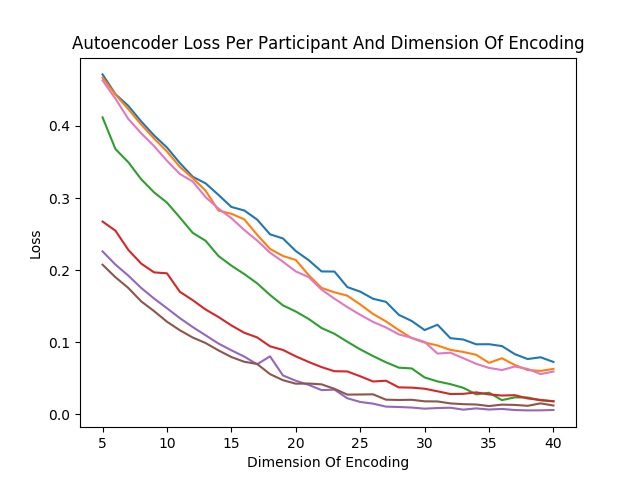
\includegraphics[width=\textwidth]{Autoencoder_loss}
	\end{minipage}
	\begin{minipage}{0.495\textwidth}
		\centering
		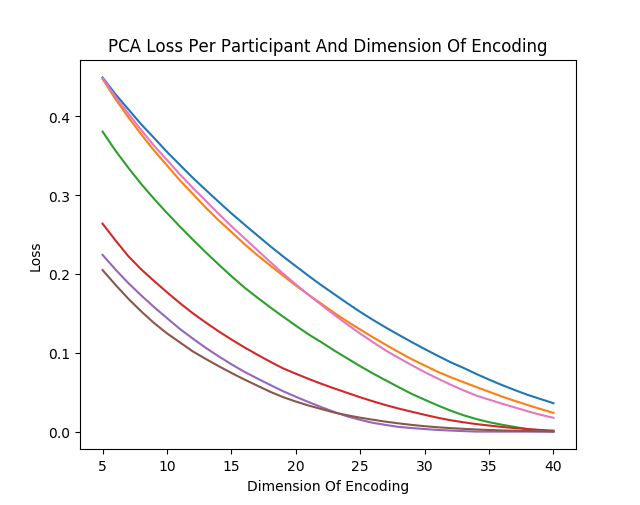
\includegraphics[width=\textwidth]{pca_loss}
	\end{minipage}
	\caption{Reconstruction loss calculated with MSE for each participant. On the left side for the autoencoder and on the right side for the PCA method}
	\label{ae_pca_loss}
\end{figure}

An investigation of the reconstruction loss for the autoencoder and PCA method (Figure \ref{ae_pca_loss}) revealed, that not only the performance of the respective model is similar, but also their reconstructional behavior. This means the aspect of linearity or non-linearity in dimensionality reduction does not have any influence on the feature set. Furthermore it can be seen, that there is a high variance for different participants in the loss function.\\
For the following experiments the choice for the feature extraction method fell in favor for taking only the finger sensors since they showed the most stable results. Also for further investigations the evaluation will be reduced to the tactile modality as there could no improvement be seen for the merged modality or only the joint angles.
%For this first problem, four different classifiers were used to test the classification accuracy. In the table below the parameters resulting in the best performance for this task are listed:
%The results for the classifiers that were trained on the target objects only is shown in Figure \ref{tvt}. The score was calculated by averaging the accuracy scores of each participant. The blue bars show the result for the tactile data and the red bars for the merged set that includes joint angles. Also shown is the standard deviation. Figure \ref{dvd} shows the same experiment but this time trained on the distractor objects. For the feature vector 20 principle components yielded the best result as Figure \ref{PCA} shows. It also presents the effect of scaling the data which shows a significant increase of the accuracy.\\
%The results show that for the target data it is possible to classify the five stimuli based on their tactile patterns with an accuracy up to 70\% with the random forest classifier and up to 60\% with the other classifier. Adding the joint angles to the data set however resulted in an small accuracy loss rather than increase.\\
%Comparing these outcomes with the classifier that were trained on the distractor data set, one can see that the performance decreases strongly on latter experiment. Considering a random walk for five classes at 20\%, the models performed just slightly better than it. Interesting is that this time the merged set with joint angles outperformed the solely tactile one in three cases.\\     
%The high variance in both results is based on the participants. The accuracy on some of their data was significantly worse than on other ones. Nonetheless a general trend could be seen for all participants which shows that the random forest classifier performed best in most cases. This model was chosen together with the 20 components for the feature vector for the following experiments.\\ 
%Overall this outcome shows that tactile patterns can be used to classify objects and that the model performs much better on the target data which was assumed. This brings up the hypotheses that rather than as individual objects, humans classify distractors as one class containing mostly object features that does't match the target they searched for. This would at least explain why the classifiers could not really separate the distractor objects. In the following experiments further investigation on this effect will be made. 

\begin{figure}[H]
		\centering
		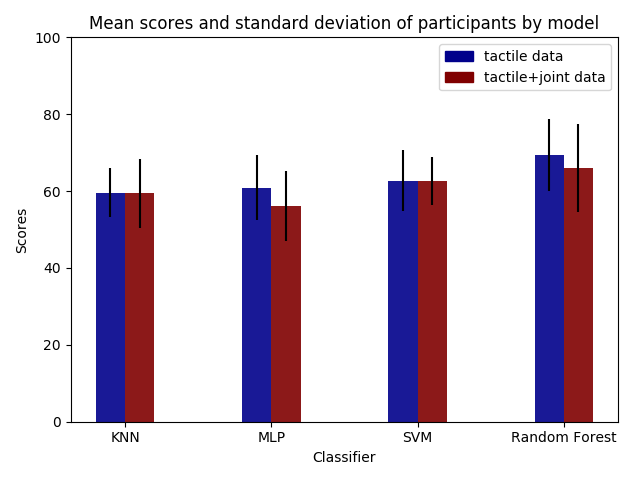
\includegraphics[width=0.9\textwidth]{TvT}
		\caption{Scores of the MLP trained on target data with various feature extraction methods}
		\label{tvt}
\end{figure}
\begin{figure}[H]
		\centering
		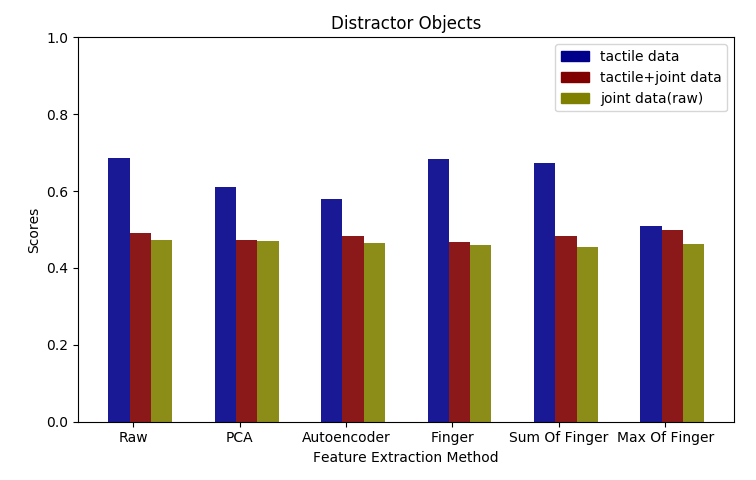
\includegraphics[width=0.9\textwidth]{DvD}
		\caption{Scores of the MLP trained on distractor data with various feature extraction methods}
		\label{dvd}
\end{figure}


\subsection{Classifying a Single Object as Either Target or Distractor}
This problem is an extension to the previous discussed one. It was found a compelling difference exist in the data regarding the role of an object. For further examinations this problem aimed at finding out whether a classifier can find the role of an object based on the generated tactile data from the exploration. To limit this problem to one model, only the random forest classifier was used as it was chosen in \ref{e2} to be the best performing model. \\
Figure \ref{tnt} shows the result of classifying single objects as either target or distractor during the experiment for each stimuli. The accuracy is composed of the mean scores of the respective objects trained separately on the data for each participant. The outcome shows high scores for all object types, especially the sphere. Again the merged data set performs slightly worse and high variances can be found for the participants.\\
These information proves that the glove can capture the crucial features that determine the objects role in the haptic search and it can be classified with reliable results. Furthermore the outperforming results of the sphere object show additional hints that the assumption from \ref{e2} might be accurate. This stimuli has high differences in its shape compared to the other ones. This means that when this object was a distractor, it was easy for participants to classify it as such. This is reflected by this result since the target and distractor role is well separable in this case as it is for humans. 

\begin{figure}[H]
	\makebox[\textwidth][c]{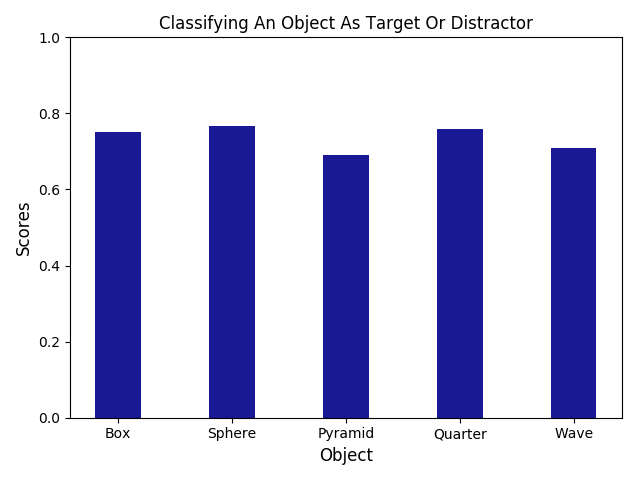
\includegraphics[scale=0.6]{TnT}}
	\caption{Mean scores of random forest trained on all participants separately by object}
	\label{tnt}
\end{figure}

\subsection{Classifying whole Data into Roles}
The aim of the last experiment is to find out if all of these assumed features that indicate for a distractor or target object can be separated as just those classes. This would be an additional evidence for the hypotheses that humans classify distractor objects in merely one class rather than the classes of the individual objects themselves as they do for targets. Figure \ref{tvd} shows the results for this experiment. Despite the fact that the distractor objects could not really be separated from each other as \ref{e2} showed, they surely can be discriminated from the target class to at least some degree. The scores of the participants show performance better than random walk, up to 68\%. This outcome reinforces the assumption. Again the merged data set doesn't show significant better scores.

\begin{figure}[H]
	\makebox[\textwidth][c]{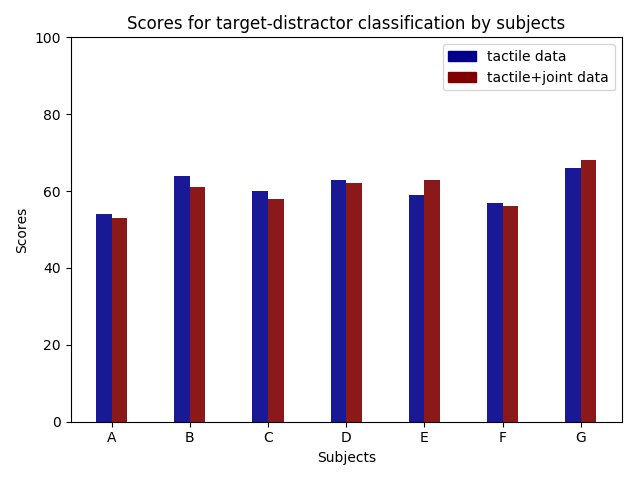
\includegraphics[scale=0.6]{TvD}}
	\caption{Scores of the random forest classifier for the two class classification problem to separate target and distractor data}
	\label{tvd}
\end{figure}
% Chapter 6

\chapter{Conclusion} % Main chapter title

\label{Conclusion} % For referencing the chapter elsewhere, use \ref{Chapter1} 
%----------------------------------------------------------------------------------------
In this work 

%----------------------------------------------------------------------------------------
%	THESIS CONTENT - APPENDICES
%----------------------------------------------------------------------------------------

\appendix % Cue to tell LaTeX that the following "chapters" are Appendices

% Include the appendices of the thesis as separate files from the Appendices folder
% Uncomment the lines as you write the Appendices

%\chapter{Experimental Instructions} \label{AppendixA}

\begin{figure}[H]
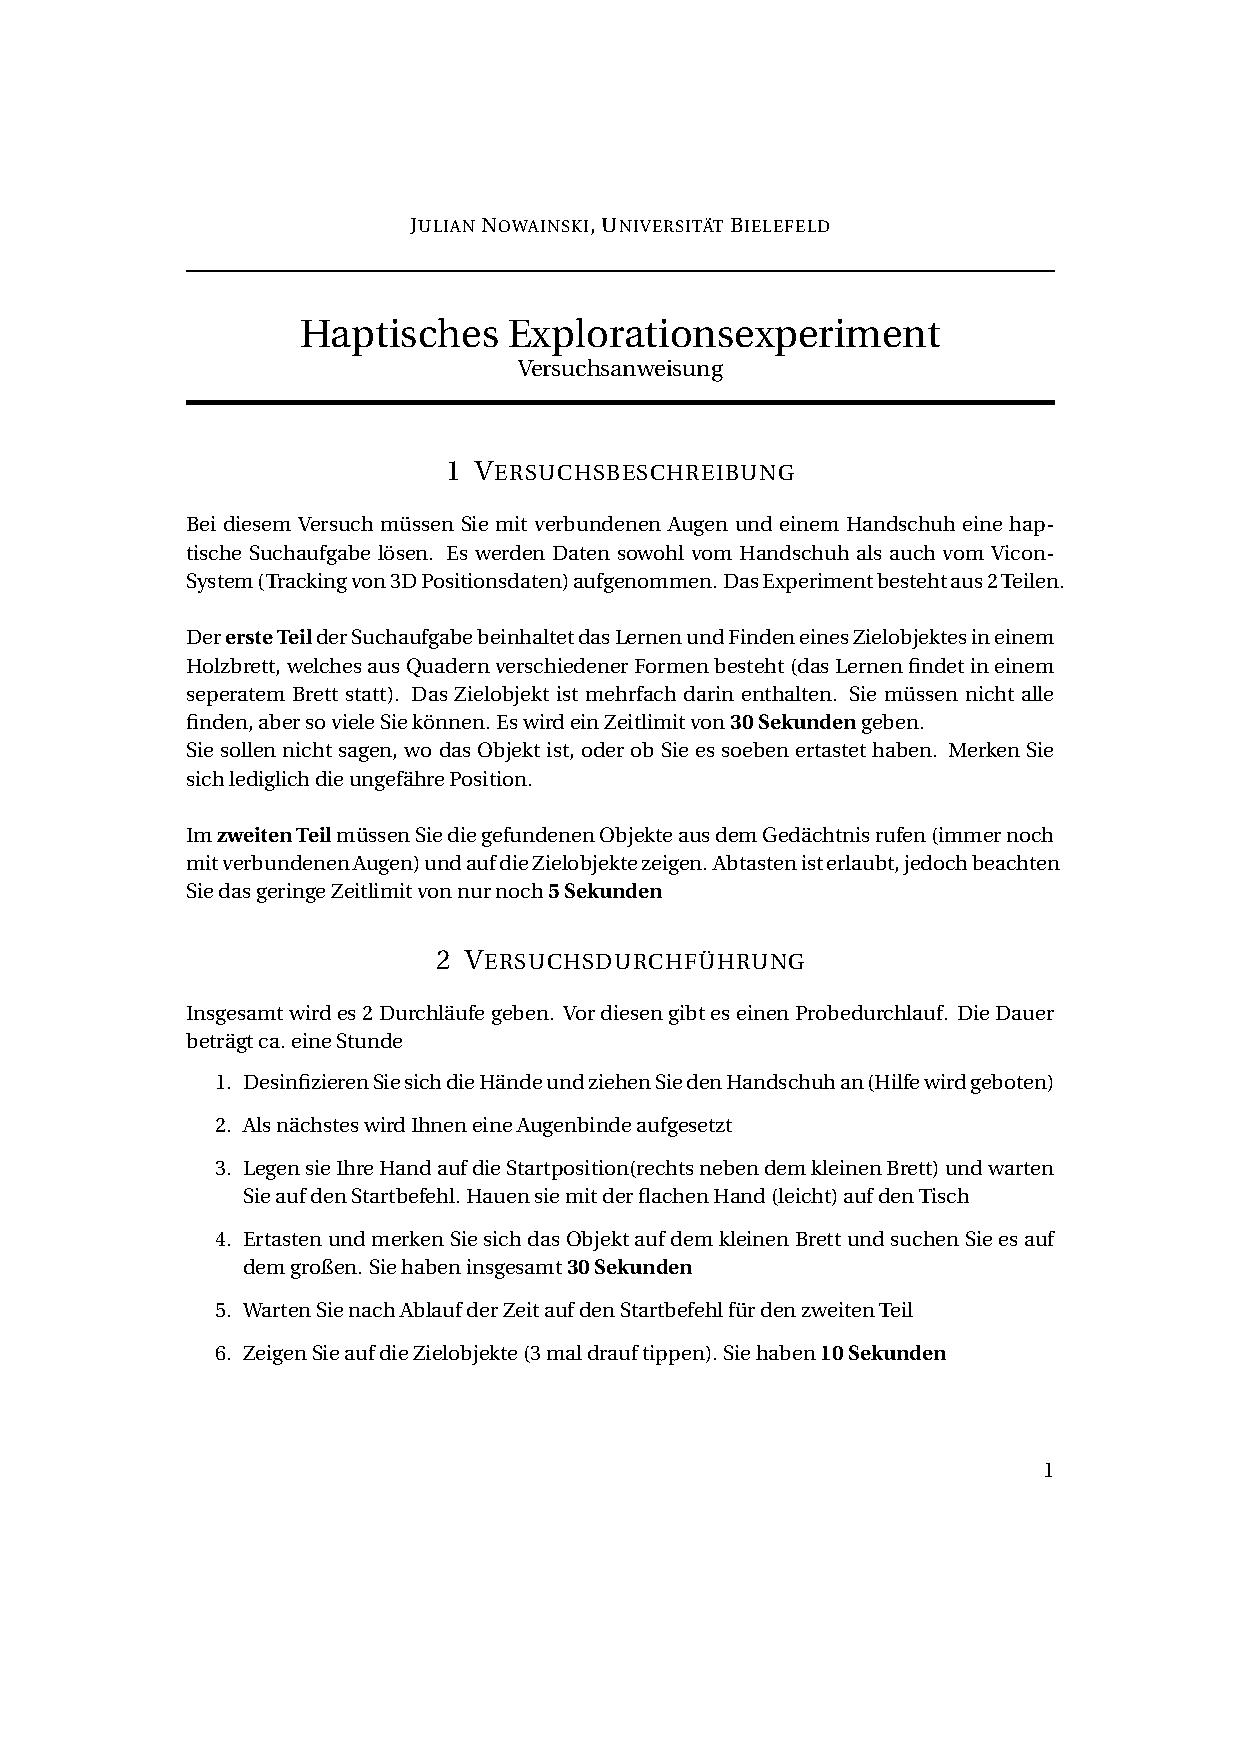
\includepdf[scale=0.9,offset=0 -80]{Appendices/instructions_ger.pdf}
\end{figure}





%\include{Appendices/AppendixB}
%\include{Appendices/AppendixC}

%----------------------------------------------------------------------------------------
%	BIBLIOGRAPHY
%----------------------------------------------------------------------------------------

\printbibliography[heading=bibintoc]

%----------------------------------------------------------------------------------------

\end{document}  
